% --- PREAMBLE ------------------------------------------------------------------
\documentclass[9pt,twocolumn,twoside]{pnas-new} % 'lineno' if desired twocolumn,
\templatetype{pnasresearcharticle} % Choose template 
\usepackage{siunitx}
\usepackage{nameref} % Cross-reference name of section
\usepackage[misc]{ifsym} % For the \Letter symbol
\usepackage{blindtext}
\DeclareGraphicsExtensions{.png,.pdf} %

% TITLE-PAGE SPECIFIC 
\title{Representation of Choices, Outcomes, and Context by Four Cell Types of the Medial Frontal Cortex}

% AFFILIATIONS
\author[1,\Letter]{Michael J. Siniscalchi}
\author[2]{Mark Dibbs}
\author[1,2,\Letter]{Alex C. Kwan}
\affil[1]{Interdepartmental Neuroscience Program, Yale University, New Haven, CT 06510, USA}
\affil[2]{Department of Psychiatry, Yale School of Medicine, New Haven, CT 06510, USA}

% SURNAME OF LEAD AUTHOR FOR RUNNING FOOTER
\leadauthor{Siniscalchi} 

% SIGNIFICANCE STATEMENT
\significancestatement{Authors must submit a 120-word maximum statement about the significance of their research paper written at a level understandable to an undergraduate educated scientist outside their field of speciality. The primary goal of the significance statement is to explain the relevance of the work in broad context to a broad readership. The significance statement appears in the paper itself and is required for all research papers.}

% AUTHOR CONTRIBUTIONS
\authorcontributions{M.J.S. and A.C.K. conceived and designed the study; M.J.S. conducted all experiments; M.J.S. and M.D. analyzed the data; M.J.S. drafted the manuscript; and M.J.S and A.C.K. revised the manuscript.}
\authordeclaration{The authors declare no competing interests.}
%\equalauthors{\textsuperscript{1}A.O.(Author One) contributed equally to this work with A.T. (Author Two) (remove if not applicable).}
\correspondingauthor{\textsuperscript{\Letter}To whom correspondence should be addressed. E-mail: michael.siniscalchi@yale.edu or alex.kwan@yale.edu}

% KEYWORDS
\keywords{decision making $|$ sensorimotor $|$ flexibility $|$ two-photon imaging} 

% ABSTRACT
\begin{abstract}
Adaptive behavior requires the flexible use of information based on learned contingencies in the environment. In rodents, the medial frontal cortex (MFC) may function importantly in this process---in part, by representing information related to choices, outcomes, and the context in which decisions are made. However, we lack a detailed understanding of how cortical microcircuits process information during context-dependent behavior. One important basic question regards how this labor is divided between different cell types of the neocortex. We used two-photon calcium imaging during a rule-switching task to separately examine the contributions of PV-, SST-, and VIP-expressing inhibitory neurons, as well as pyramidal excitatory neurons, to the representation of information required for flexible sensorimotor behavior. All four cell types were significantly modulated by choices and their outcomes, as well as the rules dictating which sensorimotor mappings would lead to a reward.
\end{abstract}

% Possibly, end with a broad comparison between PYR and GABAergic (or subsets) with regard to selectivity or preference.

% ?This could be INTRO material:
%Recent studies have focused on the question of how this labor is divided between non-overlapping cell types of the neocortex, such PV-, SST-, and VIP-expressing inhibitory neurons, as well as pyramidal excitatory neurons. Determining how distinct cell types in MFC are modulated by task variables would contribute importantly to our understanding of how MFC processes task-related information. In general, studies have emphasized differences, eg,... distinct behavioral correlates associated with the activity of different cell types.

% ? Motivate last sentence with something like:
% Differences in how distinct cell types in MFC are modulated by task variables would contribute importantly to our understanding of how MFC processes task-related information.

%In the present study, we examine the contributions of PV, SST, VIP, and PYR neurons in MFC to the representation of information required for flexible sensorimotor behavior.

%We used two-photon calcium imaging to explore whether neural representations during a rule-switching task exhibit cell-type specificity.

% One important basic question regards how this labor is divided between different cell types of the neocortex, such PV-, SST-, and VIP-expressing inhibitory neurons, as well as pyramidal excitatory neurons. In the present study, we examine the contributions of these four non-overlapping, genetically defined cell types to task-related neural representations in MFC.



\dates{This manuscript was compiled on \today}
\doi{\url{www.pnas.org/cgi/doi/10.1073/pnas.XXXXXXXXXX}} %REPLACE w BioRxiv/date on every page.

% --- MAIN SECTIONS -------------------------------------------------------------

\begin{document}

% GENERATE TITLE INCLUDING AFFILIATIONS
\maketitle 
\thispagestyle{firststyle}
\abscontent %Abstract

% MAIN TEXT

%No "Introduction" Heading; instead, try to used lettrine for large first letter style.
%\section*{Introduction} 
\dropcap{T}{he} first sentence of the introduction. \Blindtext
\section*{Results}

%\subsection*{Two-Choice Rule Switching Task}
Eighteen adult male mice were trained to high proficiency on a two-choice sensorimotor decision making task under head fixation (Fig. \ref{fig:Fig1}A--B). The task consisted of a set of trials in which subjects could choose between two stainless steel lick-ports placed on either side of the mouth, only one of which (the target) would provide a water reward when chosen. A sound cue presented at the start of each trial---either an upsweep or downsweep---indicated the target side (left for upsweeps, right for downsweeps).

\begin{figure}[htbp]

\begin{center}
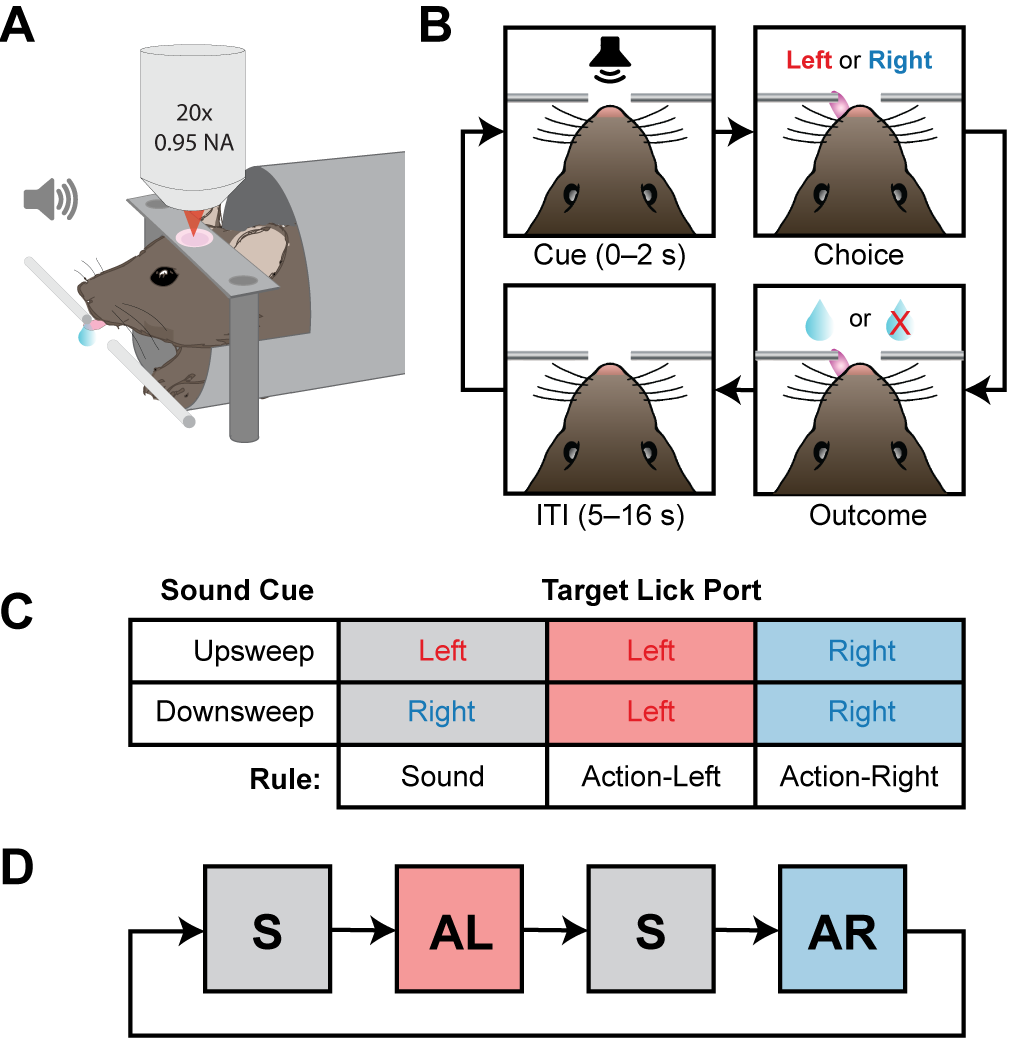
\includegraphics[width=8.7cm]{Figures/Fig1.png} 
\end{center}

\caption[Rule switching task for head-fixed mice.]
{Rule switching task for head fixed mice. (A) Experimental setup for two-choice sensorimotor task with simultaneous two-photon imaging. Mice rested inside of a stainless steel tube, with the head immobilized using a cranial implant. Two lick ports were placed on either side of the mouth to deliver water rewards. (B) Flow diagram of trial structure. A sound cue was played at the start of each trial, indicating the target port that would be rewarded (left or right). To obtain the reward, subjects were required to lick the target within 2 s following cue onset. After a random intertrial interval (ITI) of 5--16 s, a new sound cue was presented, providing a fresh opportunity to lick for a reward. (C) Table indicating the target lick port signified by each sound cue in each rule context. (D) Flow diagram of session structure. Trials governed by each rule were organized into blocks. Sound blocks (S) were interleaved with action blocks that alternated between the action-left (AL) and action-right (AR) rule. A new rule block was initiated on the next trial after an accuracy criterion was met (85\% for the past 20 trials of the current block).}

\label{fig:Fig1}
\end{figure}

Subjects were immediately rewarded with $\sim$ 2 \si{\uL} of water if the target port was chosen within 2 s of cue onset (a hit). Choosing the non-target port (an error) resulted in playback of a mild white noise sound. After a random interval of 5--16 seconds, the next cue was played, providing the opportunity to make another choice. New trials were generated until the subject failed to respond (missed) for twenty consecutive trials.

After meeting a performance criterion (three consecutive sessions at $>85\%$  accuracy), subjects were challenged with a modified version of this task, which was designed to elicit flexible sensorimotor decisions. Namely, the fixed relationship between each sound cue and its corresponding target was replaced with three alternative rules for action selection (Fig. \ref{fig:Fig1}C). 

In the sound rule, upsweeps signified a left target, and downsweeps signified a right target as described above. In the action-left rule, the target on every trial was the left port, regardless of whether upsweeps or downsweeps were presented. Conversely, under the action-right rule, the right port was always the target, irrespective of the auditory cue. 

Sessions were structured into alternating blocks of sound and action trials, such that each rule was enforced for at least 20 trials at a time (Fig. \ref{fig:Fig1}D). After 20 consecutive trials with $\geq 85\%$  accuracy, a rule-switch would occur---ie, a new rule block would begin on the next trial.

Subjects participated in $4 \pm 0$ sessions each (range: 2--5; $N=18$ mice), for a total of 65 sessions. Within each session, they completed an average $6 \pm 0$ rule blocks over the course of $561 \pm 21$ trials (all descriptive statistics are reported as $mean \pm SEM$; unless otherwise noted, the sample size $N$ is given by the number of sessions).

We used cellular resolution calcium imaging in layer 2/3 of M2 to separately measure the activity of SST, PV, VIP, and PYR neurons while subjects participated in the task. Imaging was restricted to the cell-type of interest in each experiment using one of three approaches. To target GABAergic interneurons (SST, PV, or VIP), we used transgenic mice that selectively express cyclic recombinase (cre) in the cell-type of interest \citep{taniguchi11}. In some cases ($N =$ 5 \emph{SST-cre} and 2 \emph{PV-cre} mice), an adeno-associated virus (AAV) encoding a cre-dependent GCaMP6s construct (AAV1-hSyn-Flex-GCaMP6s-WPRE-SV40) was injected into M2. In other cases, experimental subjects were F1 hybrids produced by crossing the cre-driver line with a second transgenic mouse line, \emph{Ai148} \citep{daigle18}, that expresses GCaMP6f in a cre-dependent manner ($N =$ 5 \emph{VIP-cre;Ai148} mice and 1 \emph{PV-cre;Ai148} mouse). To target pyramidal (PYR) neurons, we injected an AAV that encodes GCaMP6f under control of the CaMKII promoter (AAV1-CaMKII-GCaMP6f-WPRE-SV40; $N = 5$) \citep{kuchibhotla17, ali20}.

We visually identified a total of \num{5012} GCaMP\textsuperscript{+} neurons across all imaging sessions (Supplementary Table \ref{tab:expTable}). After excluding \num{1006} cells in which the baseline fluorescence was dimmer on average than that of the background (see Methods), we obtained cellular fluorescence time series from a total of 305 SST, 479 VIP, 263 PV, and 2959 PYR neurons. On average, $22 \pm 1$ SST, $25 \pm 1$ VIP, $22 \pm 2$ PV, or $148 \pm 9$ PYR neurons were included per session ($N =$ 14, 19, 12, and 20 sessions, respectively). The number of completed rule-blocks per session was similar during recordings from all cell-types, at $6 \pm 0$ for SST, VIP,  and PYR, and $7 \pm 1$ for PV ($F(3,61)=0.35$, $p=0.79$, 1-way ANOVA).      


\subsection*{Dependence of Lick Output on Task Structure}
As expected, the pattern of licking output was dependent on the task structure. Overall lick density varied based on elapsed time within the trial, as well as trial outcome (Fig. \ref{fig:Fig2}A--B). Specifically, the mean lick rate in completed trials increased from $0.8 \pm 0.1$ Hz in the 2 s prior to cue onset ("pre-cue"), to $2.6 \pm 0.1$ Hz in the 2 s following it ("post-cue"; paired $t(64) =38.9$, $p=\num{3e-46}$). The mean lick rate post-cue was higher for hits ($3.3 \pm 0.1$ Hz) than errors ($1.3 \pm 0.0$ Hz; paired $t(64) =24.6076$, $p=\num{2e-34}$),\ which likely reflects differences in consummatory licking.

\begin{SCfigure*}[][tbp]

% \begin{center}
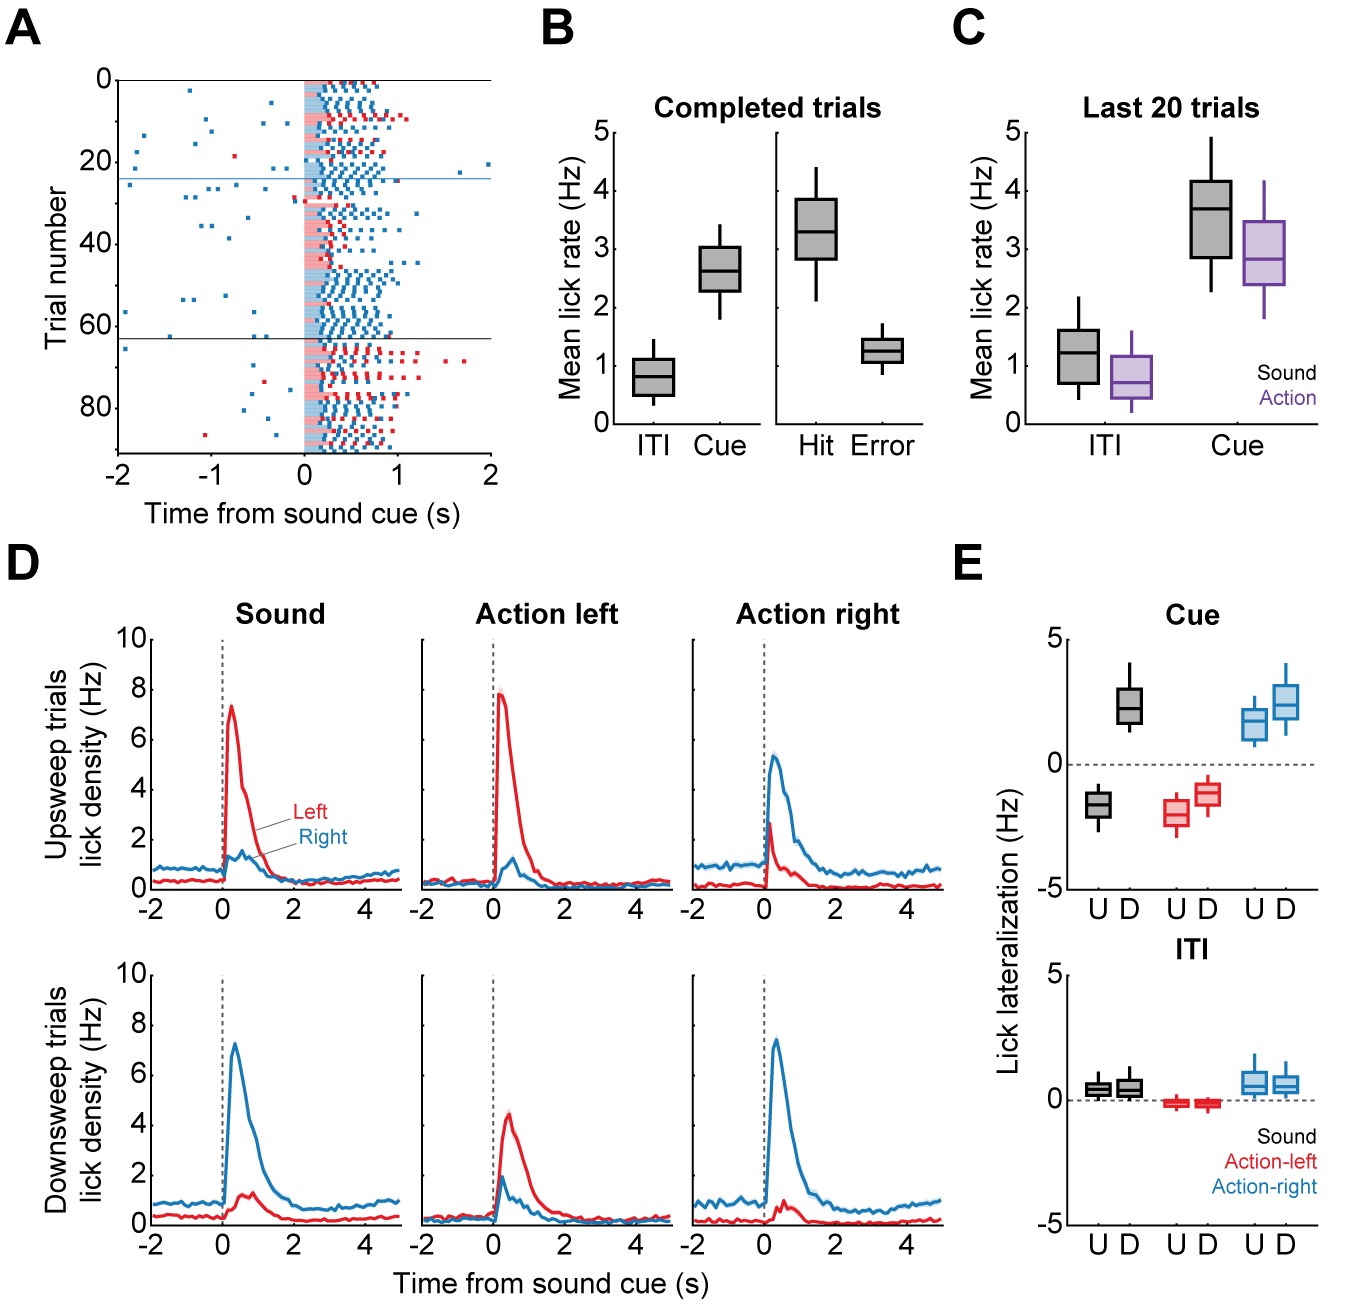
\includegraphics[width=11.4cm]{Figures/Fig2.png} 
% \end{center}

\caption[Dependence of lick output on task structure.]
{Dependence of lick output on the task structure. (A) Raster plot of individual lick times, aligned to cue onset during the first three blocks of an example session. Rows of the raster correspond to consecutive trials. The cue period of each trial is highlighted in pale red for upsweeps and pale blue for downsweeps, with red and blue tick marks representing left and right licks, respectively. Fine horizontal lines indicate the first trial of each rule block. The order of the blocks was sound--action-right--sound. (B) Mean lick rates for the 2 s periods before and after cue onset (ITI and Cue, respectively), estimated from all completed trials. Left, overall comparison of ITI and cue periods. Right, comparison of hit and error trials during the cue period. (C) Mean lick rates for the ITI and cue periods, presented separately for sound (black) and action trials (purple). (D) Mean lick density at the left (red) and right port (blue) across all sessions, calculated in 100 ms time bins surrounding cue onset. Data are plotted separately for upsweep (top) and downsweep trials (bottom) within each block type. Shading, SEM. (E) Lick lateralization in upsweep (U) and downsweep trials (D) within each block type. Lick lateralization was calculated as the difference between the number of right and left licks during the 2 s before (bottom) and after cue onset (top) in each trial. Positive and negative values indicate a greater number of right and left licks, respectively. For B--E, $N = 65$ sessions. For C--E, analysis was restricted to the last twenty trials of each block: the period in which the accuracy criterion was met. Box-and-whisker plots in all figures indicate the 9th, 25th, 50th, 75th, and 91st percentiles for each group.}

\label{fig:Fig2}
\end{SCfigure*}


An important difference between sound and action trials is that a conditional mode of action selection \citep{mitz91} is optimal under the sound rule; ie, only under the sound rule should choices depend on the identity of the sound cue. By contrast, the two action rules prescribe an unconditional mode of action selection that does not depend on cue identity. Therefore, in principle, correct choices could be made and even acted upon prior to cue onset in action trials, leading to rule-dependent differences in anticipatory licking.

To examine differences across rule types, we limited our analyses to the last twenty trials of each rule block---the period where at least 85$\%$  of choices were consistent with the corresponding rule. The mean pre-cue lick rate in action trials ($0.9 \pm 0.1$Hz) was no greater than in sound trials ($1.2 \pm 0.1$Hz; Fig. \ref{fig:Fig2}C). Moreover, the mean lick rate increased substantially upon cue onset in both sound and action trials (sound: $\Delta=2.4$Hz, paired $t(64) =29.0$, $p=\num{2e-38}$; action: $\Delta=2.0$ Hz, paired $t(64)=29.9$, $p=\num{3e-39}$). Thus, the overall pattern of licking output was largely conserved across rule types, despite fundamental differences in their temporal constraints on action selection (Fig. \ref{fig:Fig2}D).

Sound, action-left, and action-right rules are defined by the instructive content of each sound cue. Specifically, upsweeps and downsweeps signify diverging targets during sound blocks (left vs. right), and convergent but opposing targets during action-left and action-right blocks. Thus, choices should depend on an interaction between cue identity and the current rule. However, the choice made on a given trial concerns only the initial lick following the sound cue. To examine the extent to which the overall pattern of directional licking was structured by the task, we calculated a measure of lick lateralization by subtracting the mean left-lick rate from the mean right-lick rate during the post-cue period of each trial. For example, in sound trials, relative lick density was $-1.6 \pm 0.1$Hz following an upsweep, and $2.5 \pm 0.1$Hz following a downsweep.

We examined the dependence of this measure on cue identity, block-type, and their interaction with a 2-way repeated measures ANOVA  (Fig. \ref{fig:Fig2}E). Individual comparisons were made using Tukey’s post hoc test. As expected, this analysis revealed a significant dependence of lick lateralization on the interaction between block type and cue identity ($F(2,128)=410$, $p=\num{4e-56}$). Specifically, lick lateralization following upsweeps versus downsweeps differed most during sound blocks ($\Delta=4.1$Hz, $p=\num{1e-10}$). A much smaller difference was observed during action blocks (action-left: $\Delta=0.8$Hz, $p=\num{1.1e-10}$; action-right: $\Delta=0.8$Hz, $p=\num{1.1e-10}$). 

An\ identical analysis considering the pre-cue period revealed a small but significant  rule-dependent difference in lick lateralization (sound: $0.5 \pm 0.1$ Hz, action-left: $-0.1 \pm 0.0$ Hz, action-right: $0.7 \pm 0.1$ Hz; $F(2,128) =100$, $p=4e-27$). As expected, neither the cue identity ($F(1,64) =0.39$, $p=0.54$) nor the interaction of cue identity and block type ($F(2,128) =1.6$, $p=\num{0.22}$) were significant predictors of relative lick density during the pre-cue period.

\subsection*{Formal Measures of Task Performance}
Excluding the initial sound block, an average of $88 \pm 3$ trials were required to reach the accuracy criterion that triggered a rule switch (20 consecutive trials at $ \geq 85\%$ accuracy). Mean accuracy was slightly above criterion, at $86 \pm 0 \%$ during the final twenty trials of a rule block. Perseverative errors, defined as choices consistent with the previous rule but inconsistent with the current rule, were substantially more frequent than other errors. Specifically, $26 \pm 1$ perseverative errors and $3 \pm 0$ other errors were committed per block. The difference was significant in both sound ($\Delta=6$, paired $t(64) =8.2$, $p=\num{2e-11}$) and action blocks ($\Delta=38$, paired $t(64) =18.7$, $p=\num{1e-27}$).

\begin{figure}[htbp]

\begin{center}
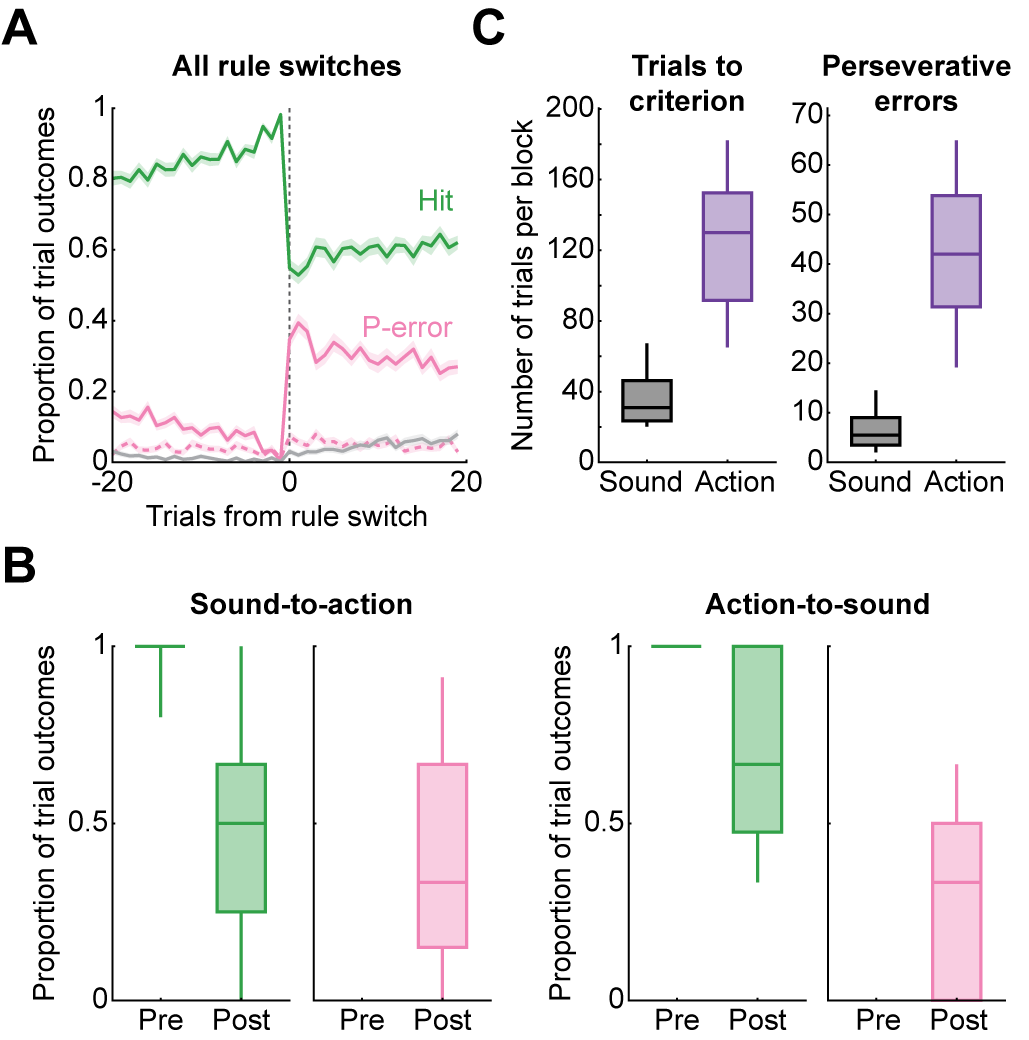
\includegraphics[width=8.7cm]{Figures/Fig3.png} 
\end{center}

\caption[Formal measures of task performance.]
{Formal measures of task performance. (A) Mean proportion of hits (green), perseverative errors (solid pink), other errors (dashed pink), and misses (gray) as a function of the number of trials from a rule switch across all sessions ($N=65$). Shading, SEM. (B) Boxplots representing the mean proportion of hits (green) and preseverative errors (pink) for trials immediately preceding a rule switch (Pre) and for trials immediately following one (Post). Results are presented separately for switches from the sound rule to an action rule (left), and vice-versa (right). (C) Boxplots representing the number of trials taken to reach criterion (left), and the number of perseverative errors committed (right), during sound (black) and action blocks (purple). All boxes indicate quartiles 1--3; whiskers indicate 9th and 91st percentiles.}

\label{fig:Fig3}
\end{figure}

As expected, accuracy dropped precipitously following a rule switch (\ref{fig:Fig3}A). The proportion of hits decreased from $98 \pm 1 \%$ in the trial before a rule switch, to $55 \pm 2 \%$ in the next trial (paired $t(64) =16.9$, $p=\num{3e-25}$). This reduction in accuracy was mostly attributable to an increase in perseverative errors, which accounted for $0 \pm 0 \%$ of trials immediately preceding a rule switch and $35 \pm 2 \%$ of trials immediately following (paired $t(64) =13.7$, $p=\num{9e-21}$). A much smaller increase was noted in the proportion of other errors ($\Delta=6\%$, paired $t(64) =3.8$, $p=\num{3e-4}$) and misses ($\Delta=3\%$, paired $t(64) =3.7$, $p=\num{5e-4}$). 

Results of this analysis are presented separately for switches from the sound rule to an action rule, and vice-versa, in Figure \ref{fig:Fig3}B. In both cases, the proportion of hits decreased substantially in the trial following a rule switch (sound-to-action: $\Delta=51\%$, paired $t(64) =12.6$, $p=\num{5e-19}$; action-to-sound: $\Delta=34\%$, paired $t(64) =8.7$, $p=\num{2e-12}$). Following a sound-to-action rule switch, the proportion of hits was indistinguishable from chance, at $46 \pm 4 \%$ ($t(64)=1.0$, $p=0.30$; one-sample t-test for the null hypothesis, $H_0:\Delta=0.5$), but remained significantly above chance following an action-to-sound rule switch: $mean=66 \pm 4 \%$, $t(64)=4.1$, $p=\num{1e-4}$). In both cases, the proportion of perseverative errors increased significantly (sound-to-action: $\Delta=39\%$, paired $t(64) =9.9$, $p=\num{1e-14}$; action-to-sound: $\Delta=29\%$, paired $t(64) =8.5$, $p=\num{4e-12}$).  

Although subjects were capable of adjusting their sensorimotor decisions to both rule types, in general, they adapted more readily during action-to-sound rule transitions than the reverse (Fig. \ref{fig:Fig3}C). During sound blocks, substantially fewer trials were taken to reach the accuracy criterion ($39 \pm 3$ vs. $126 \pm 6$; paired $t(64) =13.4$, $p=\num{3e-20}$), and fewer perseverative errors were committed before the criterion was reached ($7 \pm 1$ vs. $43 \pm 2$; paired $t(64) =14.3$, $p=\num{1e-21}$).

\subsection*{Task-Related Modulation of Neural Activity}


\subsubsection*{Choice-Related Modulation}

\subsubsection*{Outcome-Related Modulation}

\subsubsection*{Context-Related Modulation}
\input{Discussion}
% TEXT OF MATERIALS & METHODS 

\newcommand{\tg}[1]{\textsuperscript{\textit{#1}}}

\matmethods{%

\subsection*{Experimental Subjects}
Experimental subjects ($N=18$) were adult male transgenic mice from a C57BL/6J genetic background (\ref{tab:expTable}). All mice were hemizygous hybrids of the following strains purchased from the Jackson Laboratory (Bar Harbor, ME):
Sst\tg{tm2.1(cre)Zjh}/J (\emph{SST-cre}; stock no. 013044), Vip\tg{tm1(cre)Zjh}/J (\emph{VIP-cre}; stock no. 010908), B6.129P2-Pvalb\tg{tm1(cre)Arbr}/J (\emph{PV-cre}; stock no. 017320),  or B6.Cg-Gt(ROSA)26Sor\tg{tm9(CAG-tdTomato)Hze}/J (\emph{flex-tdTomato}; stock no. 007909). Six subjects were bred from B6.Cg-Igs7\tg{tm148.1(tetO-GCaMP6f,CAG-tTA2)Hze}/J mice (\emph{Ai148}; \cite{daigle18}) kindly provided by Hongkui Zeng (Allen Institute, Seattle, WA). Specifically, a total of seven \emph{PV-cre;flex-tdTomato mice}, five \emph{SST-cre;flex-tdTomato mice}, five \emph{VIP-cre;Ai148} mice, and one \emph{PV-cre;Ai148} mouse were used for our experiments.

Mice were housed in a dedicated facility administered by the Yale Animal Resource Center. Five littermates were kept together per cage, supplemented with an igloo and cotton nesting material. Room lights were turned on from 7 am until 7 pm. Training and experiments were conducted outside of the facility between the hours of 10 am and 6 pm. All experimental procedures were approved by the Institutional Animal Care and Use Committee of Yale University.


\subsection*{Rule Switching Task}
% bias_factor = double(hit_rates[1] - hit_rates[2])/double(100);
% 		temp = random()*double(2) + bias_factor;

% Mice were secured inside a... using an implanted headplate to an apparatus consisting of…
% Mice were seated in a XX-mm-diameter tube…

% Eighteen adult male mice were trained to high proficiency on a two-choice sensorimotor decision making task under head fixation (Fig. \ref{fig:Fig1}A--B). The task consisted of a set of trials in which subjects could choose between two stainless steel lick-ports placed on either side of the mouth, only one of which (the target) would provide a water reward when chosen. A sound cue presented at the start of each trial---either an upsweep or downsweep---indicated the target side (left for upsweeps, right for downsweeps).

% Subjects were immediately rewarded with $\sim$ 2 \si{\uL} of water if the target port was chosen within 2 s of cue onset (a hit). Choosing the non-target port (an error) resulted in playback of a mild white noise sound. After a random interval of 5--16 seconds, the next cue was played, providing the opportunity to make another choice. New trials were generated until the subject failed to respond (missed) for twenty consecutive trials.

% After meeting a performance criterion (three consecutive sessions at $>85\%$  accuracy), subjects were challenged with a modified version of this task, which was designed to elicit flexible sensorimotor decisions. Namely, the fixed relationship between each sound cue and its corresponding target was replaced with three alternative rules for action selection (Fig. \ref{fig:Fig1}C). 

% In the sound rule, upsweeps signified a left target, and downsweeps signified a right target as described above. In the action-left rule, the target on every trial was the left port, regardless of whether upsweeps or downsweeps were presented. Conversely, under the action-right rule, the right port was always the target, irrespective of the auditory cue. 

% Sessions were structured into alternating blocks of sound and action trials, such that each rule was enforced for at least 20 consecutive trials at a time. After 20 consecutive trials with at least 85$\%$  accuracy, a rule-switch would occur---ie, a new rule block would begin on the next trial.

\subsection*{Cell Type Specific Imaging}
We used two-photon calcium imaging to monitor neural activity at cellular resolution while mice participated in the rule switching task. To separately measure the activity of somatostatin- (SST; $N=309$ cells from 5 mice), parvalbumin- (PV; $N=263$ cells from 3 mice), and vasointestinal peptide-expressing (VIP; $N=488$ cells from 5 mice) interneurons, as well as CamKIIa-expressing excitatory neurons (PYR; $N=3952$ cells from 5 mice), we took three different approaches which have all been validated in earlier studies.

To image the activity of SST and PV neurons, a cyclic recombinase- (cre) dependent adeno-associated virus encoding GCaMP6s (AAV1-hSyn-Flex-GCaMP6s-WPRE-SV40, Penn Vector Core) was injected intracranially in hybrid reporter mice (SST::tdTomato or PV::tdTomato) that express both cre and the orange fluorescent protein, tdTomato, selectively in the cell-type of interest \citep{taniguchi11, ali20}. Neuronal expression of tdTomato was aimed at providing a frame-by-frame anatomical reference channel to be used later for movement correction of data from the activity-dependent (GCaMP) channel. 

To monitor VIP and PV neurons, we bred VIP::GCaMP6f and PV::GCaMP6f hybrid reporter mice, which selectively express GCaMP6f in the cell-type of interest \citep{daigle18,devries20}. 
To monitor pyramidal neurons, five PV-cre::tdTomato mice were injected intracranially with an AAV encoding GCaMP6f under control of the CaMKII-promoter (AAV1-CaMKII-GCaMP6f-WPRE-SV40, Penn Vector Core; \cite{kuchibhotla17,ali20}). 

\subsubsection*{Intracranial Injections and Cranial Window Implantation}
Subjects were treated preoperatively with analgesic and antiinflammatory drugs (carprofen, 5 mg/kg, SC, \#024751, Butler Animal Health; and dexamethasone, 3 mg/kg, SC, Dexaject SP, \#002459, Henry Schein Animal Health). Anesthesia was induced with 2\% isoflurane in oxygen, and then gradually reduced to 1--1.5\% for the remainder of the procedure. A water-circulating heating pad (Gaymar Stryker) was placed under the animal’s body, and maintained at 38\si{\celsius}.

After stabilizing the head in a stereotaxic frame with ear bars (David Kopf Instruments), the scalp was shaven and cleaned with Betadine (Perdue Products L.P.). The surface of the skull was then exposed through a midsagittal incision extending from the interaural line to the level of the orbits. The periosteum was removed, and the skull cleaned, by scrubbing briefly with 3\% hydrogen peroxide on a cotton swab. All contacted tissue was then rinsed immediately with artificial cerebrospinal fluid (aCSF; in mM: 5 KCl, 5 HEPES, 135 NaCl, 1 MgCl$_2$, 1.8 CaCl$_2$; pH 7.3).

A 3-mm-diameter circular craniotomy, centered approximately over the target location in M2 (AP, $bregma + 1.5$ mm; ML, $bregma - 0.5$ mm), was made using a 400-\si{\um}-diameter spherical bur attached to a Foredom dental drill. The circumscribed section of skull was then carefully removed with fine forceps to expose the dura. A small cube of Gelfoam (McKesson), presaturated with aCSF, was immediately applied to ensure hemostasis. Several additional cubes of saturated Gelfoam were used to gently cleanse the dural surface of any debris.

For procedures requiring intracranial AAV injections, a fine-tipped glass micropipette was secured to a microinjection system (Nanoject II, Drummond) and front-filled with ~1.5 \si{\uL} of the viral suspension. All viruses were stored as frozen aliquots, and diluted to approximately 1012 genome copies per mL in PBS prior to injection. Four injections were made, forming a 200-\si{\um}-wide square centered on the target location. Approximately 46 nL were injected into each site, at a depth of 400 \si{\um} below the dura. After the last injection, the dura was cleaned thoroughly with saturated Gelfoam.

A glass window implant was then fit to the craniotomy and glued to the surrounding skull surface. The implant consisted of five concentric, \#1 thickness, circular glass coverslips (Warner Instruments) joined with an optical adhesive (NOA 61, Norland). The superficial layer was wider than the remaining layers (4- vs. 3-mm-diameter), to form a lip that could be attached to the skull. Prior to implantation, the window was swabbed thoroughly with 90\% ethanol and then rinsed with aCSF. After flooding the craniotomy with aCSF, the implant was lowered into place and secured with a high-viscosity adhesive (Loctite 454). After allowing ~10 min for the adhesive to cure, a custom-made stainless steel headplate (eMachineShop.com) was cemented to the skull with C\&B Metabond (Parkell). Care was taken to cover any exposed bone.

Subjects were treated post-operatively with carprofen (5 mg/kg, SC), diluted to 0.17 mg/mL in 0.9\% preservative-free saline (Hospira) for fluid support. The treatment was repeated twice daily for three days following the surgery, along with a daily injection of dexamethasone (3 mg/kg, SC). At least one full week was allowed for recovery prior to behavioral training.

\subsubsection*{Two-Photon Imaging}
To image neural activity at cellular resolution in vivo, an ultrafast laser beam (Chameleon Ultra II, Coherent) was focused on the brain tissue through a water immersion objective (XLUMPLFLN, 20X/0.95 NA; Olympus) attached to a Movable Objective Microscope (Sutter Instrument). Ultrasound gel (\#9004352SM, Henry Schein) was applied to the cranial window as an immersion medium, to prevent a gradual image degradation observed in earlier experiments due to evaporation.
Excitation power after the objective was adjusted using a Pockels cell (350-80-LA-
02; Conoptics), up to a maximum of 100 mW. Emitted fluorescence was split between two channels and bandpass filtered at center wavelengths of 525 nm (GCaMP6) and 605 nm (tdTomato) prior to collection by a set of GaAsP photomultiplier tubes (H7422P-40MOD; Hamamatsu). Excitation wavelength was set to 1020--1050 nm for most experiments, in order to optimize the GCaMP6:tdTomato emission ratio. For single-channel GCaMP6 imaging, an excitation wavelength of 940 nm was used.

Image acquisition was controlled by the ScanImage package for MATLAB \citep{pologruto03}. Time-lapse images of the field-of-view were acquired using a bidirectional raster scan at 1kHz. Each imaging frame contained 256 × 256 pixels, for a nominal frame rate of 3.62 Hz including flyback time. Frames from each behavioral trial were saved separately in multi-page tagged image file format (TIFF). Imaging and behavioral data were synchronized by assigning an external trigger in ScanImage to a TTL pulse sent by NBS Presentation at the start of each trial. Upon receiving the trigger, ScanImage would write the current frame to the first page of a new TIFF. A timestamp for the trigger would be recorded in the TIFF header, as well as in a text file logged by Presentation.        

The target imaging location in M2 was found before each session as follows. The AP coordinate (bregma+1.5mm) was approximated by centering the field-of-view (FOV) on a small dot that had been marked in permanent ink along the perimeter of the cranial window during stereotaxic surgery surgery. The ML coordinate (bregma-1.5mm) was approximated by centering the FOV on the superior sagittal sinus and then subtracting 500 \si{\um}. Some deviations from these coordinates were permitted, eg, in cases of occluding blood vessels, but all FOVs analyzed were centered within 200 \si{\um} of the target location. The approximate anatomical depth of each FOV was estimated as the distance from a focal plane centered on the dura directly above it, calculated from the corresponding depth measurements displayed on the microcontroller. Depth ranged 212--415 \si{\um} for SST sessions (mean: 228 \si{\um}, $N=14$), 109--216 for VIP sessions (mean: 175 \si{\um}, $N=19$), 215--383 for PV sessions (mean: 292, $N=12$), and 170--278 for PYR sessions (mean: 219, $N=20$). Brain tissue was not analyzed post-mortem to confirm the estimated imaging locations, but all fields-of-view were assumed to be within layers 2/3 of M2.

\subsection*{Analysis of Behavioral Data}
\subsection*{Analysis of Imaging Data}
\subsubsection*{Movement Correction}
\subsubsection*{Cellular Fluorescence Measurements}
\subsubsection*{Alignment and Trial Averaging}
\subsubsection*{Modulation of Neural Activity by Task Variables}

\subsection*{Statistics}
All statistics were computed in MATLAB.

Descriptive statistics are reported either as the \emph{sample} $mean \pm SEM$, or as the sample median and interquartile range (IQR), at a precision consistent with the primary data. For all analyses, point estimates were calculated as the mean within each session, and the sample size $N$ was given by the number of sessions considered. 

For behavioral comparisons, the sampling distribution for the mean difference across groups was assumed to be normal. No explicit test of normality was performed. However, the sample size  ($N=65$) was sufficiently large to rely on parametric statistics. Specifically, a paired t-test was used for comparisons across two groups (eg, hit vs. error trials). For comparisons across sound, action-left, and action-right blocks, a repeated measures model was fit to the data using the function \texttt{fitrm}, with the session index included as the only between-subjects factor. A two-way, within-subject design was used to assess the main effects of \emph{cue} and \emph{block-type}, as well as any \emph{cue} $\times$ \emph{block-type} interaction. All $F$-statistics were estimated by feeding the parameters of the model into the function \texttt{ranova}.

Neural preference and selectivity measures were compared to null results generated using shuffled trial types. These comparisons were made within each cell type, and hence sample sizes were smaller (range: 12--20 sessions). Additionally, the empirical distributions were often notably skewed, with unequal variances relative to the corresponding null distribution. Therefore, a signed-rank test was used for these comparisons. For comparisons across multiple cell types we used the Kruskal-Wallis $H$-test, followed by Tukey's post hoc method for multiple comparisons. 

}% 

\showmatmethods{} % Display the Materials and Methods section

% ACKNOWLEDGMENTS
\acknow{We thank Hongkui Zeng for providing \emph{Ai148} transgenic mice. The authors received financial support from the National Institute of Mental Health (grants R01MH112750 and R21MH118596 to A.C.K.) and the National Science Foundation Graduate Research Fellowship (DGE-1122492 to M.J.S.)}
\showacknow{} % Display the acknowledgments section

% BIBLIOGRAPHY
\section*{Bibliography}
\bibliography{Bibliography}

% SUPPLEMENTS
\onecolumn

% Tables
% Table generated by Excel2LaTeX
\begin{table*}[htbp]
  \centering
  \caption{Summary of Experiments}
  \begin{tabular}{lccccccc}
          & Experiment\_ID & Strain & Virus &  \# Trials & \# Blocks & \# Cells & \# Excl. \\
          \midrule
    1     & 170928 M47 & SST-cre & AAV1-flex-GCaMP6s & 597   & 7     & 17    & 0 \\
    2     & 171012 M47 & SST-cre & AAV1-flex-GCaMP6s & 485   & 6     & 21    & 0 \\
    3     & 171114 M47 & SST-cre & AAV1-flex-GCaMP6s & 420   & 5     & 32    & 0 \\
    4     & 171024 M47 & SST-cre & AAV1-flex-GCaMP6s & 372   & 4     & 19    & 0 \\
    5     & 171103 M47 & SST-cre & AAV1-flex-GCaMP6s & 361   & 5     & 30    & 0 \\
    6     & 170929 M48 & SST-cre & AAV1-flex-GCaMP6s & 453   & 6     & 17    & 0 \\
    7     & 171013 M48 & SST-cre & AAV1-flex-GCaMP6s & 624   & 7     & 15    & 0 \\
    8     & 171112 M49 & SST-cre & AAV1-flex-GCaMP6s & 457   & 4     & 27    & 0 \\
    9     & 171101 M49 & SST-cre & AAV1-flex-GCaMP6s & 395   & 4     & 23    & 3 \\
    10    & 171011 M50 & SST-cre & AAV1-flex-GCaMP6s & 724   & 7     & 14    & 0 \\
    11    & 171014 M50 & SST-cre & AAV1-flex-GCaMP6s & 741   & 6     & 22    & 0 \\
    12    & 171027 M50 & SST-cre & AAV1-flex-GCaMP6s & 487   & 5     & 27    & 0 \\
    13    & 171103 M51 & SST-cre & AAV1-flex-GCaMP6s & 702   & 6     & 24    & 0 \\
    14    & 171109 M51 & SST-cre & AAV1-flex-GCaMP6s & 740   & 11    & 21    & 1 \\
    15    & 180927 M57 & VIP::GCaMP6f & none  & 1025  & 7     & 29    & 0 \\
    16    & 181010 M57 & VIP::GCaMP6f & none  & 506   & 5     & 29    & 0 \\
    17    & 181012 M57 & VIP::GCaMP6f & none  & 748   & 9     & 18    & 0 \\
    18    & 181026 M57 & VIP::GCaMP6f & none  & 715   & 7     & 17    & 0 \\
    19    & 181023 M58 & VIP::GCaMP6f & none  & 408   & 6     & 23    & 0 \\
    20    & 181025 M58 & VIP::GCaMP6f & none  & 263   & 5     & 24    & 0 \\
    21    & 181030 M58 & VIP::GCaMP6f & none  & 384   & 5     & 22    & 0 \\
    22    & 181016 M59 & VIP::GCaMP6f & none  & 367   & 5     & 24    & 0 \\
    23    & 181017 M59 & VIP::GCaMP6f & none  & 617   & 6     & 17    & 0 \\
    24    & 181019 M59 & VIP::GCaMP6f & none  & 532   & 5     & 23    & 3 \\
    25    & 181024 M59 & VIP::GCaMP6f & none  & 527   & 7     & 30    & 1 \\
    26    & 181025 M59 & VIP::GCaMP6f & none  & 478   & 9     & 26    & 0 \\
    27    & 181016 M60 & VIP::GCaMP6f & none  & 636   & 6     & 31    & 0 \\
    28    & 181023 M60 & VIP::GCaMP6f & none  & 561   & 6     & 25    & 2 \\
    29    & 181025 M60 & VIP::GCaMP6f & none  & 409   & 6     & 28    & 0 \\
    30    & 181026 M60 & VIP::GCaMP6f & none  & 470   & 5     & 26    & 1 \\
    31    & 181030 M60 & VIP::GCaMP6f & none  & 437   & 4     & 34    & 2 \\
    32    & 181027 M61 & VIP::GCaMP6f & none  & 367   & 5     & 36    & 0 \\
    33    & 181031 M61 & VIP::GCaMP6f & none  & 361   & 7     & 26    & 0 \\
    34    & 171018 M42 & PV-cre & AAV1-flex-GCaMP6s & 287   & 5     & 16    & 0 \\
    35    & 171104 M42 & PV-cre & AAV1-flex-GCaMP6s & 288   & 5     & 26    & 0 \\
    36    & 171113 M42 & PV-cre & AAV1-flex-GCaMP6s & 592   & 9     & 26    & 0 \\
    37    & 171012 M43 & PV-cre & AAV1-flex-GCaMP6s & 378   & 6     & 25    & 0 \\
    38    & 171019 M43 & PV-cre & AAV1-flex-GCaMP6s & 609   & 7     & 20    & 0 \\
    39    & 171027 M43 & PV-cre & AAV1-flex-GCaMP6s & 310   & 4     & 23    & 0 \\
    40    & 171102 M43 & PV-cre & AAV1-flex-GCaMP6s & 457   & 4     & 39    & 0 \\
    41    & 190503 M62 & PV::GCaMP6f & none  & 605   & 6     & 12    & 0 \\
    42    & 190508 M62 & PV::GCaMP6f & none  & 712   & 7     & 20    & 0 \\
    43    & 190517 M62 & PV::GCaMP6f & none  & 515   & 5     & 17    & 0 \\
    44    & 190522 M62 & PV::GCaMP6f & none  & 769   & 11    & 22    & 0 \\
    45    & 190620 M62 & PV::GCaMP6f & none  & 872   & 11    & 17    & 0 \\
    46    & 181003 M52 & PV-cre & AAV1-CamKII-GCaMP6f & 701   & 4     & 158   & 38 \\
    47    & 181005 M52 & PV-cre & AAV1-CamKII-GCaMP6f & 463   & 9     & 151   & 31 \\
    48    & 181009 M52 & PV-cre & AAV1-CamKII-GCaMP6f & 453   & 4     & 151   & 35 \\
    49    & 181011 M52 & PV-cre & AAV1-CamKII-GCaMP6f & 520   & 6     & 233   & 39 \\
    50    & 180919 M53 & PV-cre & AAV1-CamKII-GCaMP6f & 693   & 6     & 206   & 49 \\
    51    & 180925 M53 & PV-cre & AAV1-CamKII-GCaMP6f & 830   & 9     & 215   & 72 \\
    52    & 180928 M53 & PV-cre & AAV1-CamKII-GCaMP6f & 694   & 7     & 157   & 31 \\
    53    & 180829 M54 & PV-cre & AAV1-CamKII-GCaMP6f & 569   & 5     & 239   & 83 \\
    54    & 180905 M54 & PV-cre & AAV1-CamKII-GCaMP6f & 667   & 7     & 140   & 45 \\
    55    & 180912 M54 & PV-cre & AAV1-CamKII-GCaMP6f & 774   & 9     & 139   & 40 \\
    56    & 180918 M54 & PV-cre & AAV1-CamKII-GCaMP6f & 710   & 7     & 188   & 29 \\
    57    & 180921 M54 & PV-cre & AAV1-CamKII-GCaMP6f & 568   & 6     & 185   & 40 \\
    58    & 180831 M55 & PV-cre & AAV1-CamKII-GCaMP6f & 424   & 5     & 229   & 47 \\
    59    & 180905 M55 & PV-cre & AAV1-CamKII-GCaMP6f & 573   & 6     & 325   & 96 \\
    60    & 180907 M55 & PV-cre & AAV1-CamKII-GCaMP6f & 496   & 5     & 243   & 50 \\
    61    & 180918 M55 & PV-cre & AAV1-CamKII-GCaMP6f & 980   & 8     & 272   & 50 \\
    62    & 180920 M55 & PV-cre & AAV1-CamKII-GCaMP6f & 777   & 6     & 230   & 66 \\
    63    & 180830 M56 & PV-cre & AAV1-CamKII-GCaMP6f & 530   & 5     & 169   & 37 \\
    64    & 180906 M56 & PV-cre & AAV1-CamKII-GCaMP6f & 416   & 4     & 165   & 58 \\
    65    & 180921 M56 & PV-cre & AAV1-CamKII-GCaMP6f & 834   & 8     & 157   & 57 \\
    \end{tabular}%
  \label{tab:expTable}%
\end{table*}%

% \begin{table}%[tbhp]
% \centering
% \caption{Comparison of the fitted potential energy surfaces and ab initio benchmark electronic energy calculations}
% \begin{tabular}{lrrr}
% Species & CBS & CV & G3 \\
% \midrule
% 1. Acetaldehyde & 0.0 & 0.0 & 0.0 \\
% 2. Vinyl alcohol & 9.1 & 9.6 & 13.5 \\
% 3. Hydroxyethylidene & 50.8 & 51.2 & 54.0\\
% \bottomrule
% \end{tabular}

% \addtabletext{nomenclature for the TSs refers to the numbered species in the table.}
% \end{table}

\include{Figures/Table_Comparisons}


\end{document}

% --- HELPFUL INFORMATION ----------------------------------------------

% Figure Formatting from PNAS:
% Images must be provided at final size, preferably 1 column width (8.7cm). Figures wider than 1 column should be sized to 11.4cm or 17.8cm wide. Numbers, letters, and symbols should be no smaller than 6 points (2mm) and no larger than 12 points (6mm) after reduction and must be consistent. 

% To insert a figure wider than one column, please use the \verb|\begin{figure*}...\end{figure*}| environment. Figures wider than one column should be sized to 11.4 cm or 17.8 cm wide. Use \verb|\begin{SCfigure*}...\end{SCfigure*}| for a wide figure with side legends.

% Example for Table Environment:
% \begin{table}%[tbhp]
% \centering
% \caption{Comparison of the fitted potential energy surfaces and ab initio benchmark electronic energy calculations}
% \begin{tabular}{lrrr}
% Species & CBS & CV & G3 \\
% \midrule
% 1. Acetaldehyde & 0.0 & 0.0 & 0.0 \\
% 2. Vinyl alcohol & 9.1 & 9.6 & 13.5 \\
% 3. Hydroxyethylidene & 50.8 & 51.2 & 54.0\\
% \bottomrule
% \end{tabular}

% \addtabletext{nomenclature for the TSs refers to the numbered species in the table.}
% \end{table}

% Supplementary Information
% The PNAS Overleaf SI template can be found here: \href{https://www.overleaf.com/latex/templates/pnas-template-for-supplementary-information/wqfsfqwyjtsd}{here}. Refer to the SI Appendix in the manuscript at an appropriate point in the text. Number supporting figures and tables starting with S1, S2, etc.

% For Hypertext in Article:
% eg, \href{http://www.pnascentral.org/cgi-bin/main.plex}{PNAScentral}

